\documentclass[]{article}
\usepackage{caption,subcaption,graphicx,float,url,amsmath,amssymb,tocloft,wasysym,amsthm,thmtools,textcomp,listings,amsfonts,cancel}
\usepackage[hidelinks]{hyperref}
\usepackage[toc,acronym,nonumberlist]{glossaries}
\usepackage[]{algorithm2e}
\setacronymstyle{long-short}
\usepackage{glossaries-extra}
\graphicspath{{figs/}} 
\setlength{\cftsubsecindent}{0em}
\setlength{\cftsecnumwidth}{3em}
\setlength{\cftsubsecnumwidth}{3em}
\newcommand\numberthis{\addtocounter{equation}{1}\tag{\theequation}}
\newtheorem{thm}{Theorem}
\newtheorem{cor}[thm]{Corollary}
\setcounter{tocdepth}{1}
\usepackage[toc,page]{appendix}
%opening
\title{
	Computation in Complex Systems\\
	Week 2\\
	 Algorithms \& Landscapes
}

%\makeglossaries


\begin{document}

\maketitle

\tableofcontents
%\listofalgorithms
\section{Maximum independent set}

\subsection{What is the maximum value of the independent set?}

\begin{figure}[H]
	\begin{center}
		\caption{What is the maximum value of the independent set?}
		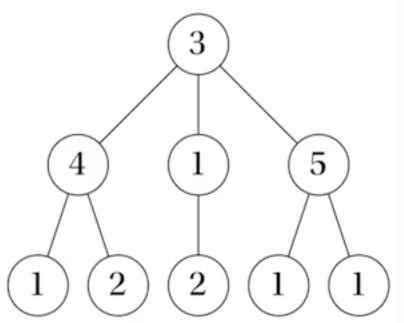
\includegraphics[width=0.6\textwidth]{mwisQ}
	\end{center}
\end{figure}

Observations:
\begin{enumerate}
	\item A tree with $N$ nodes has $2^N-1$ non empty subsets, so a brute-force search is exponential. Let's not go there!
	\item Either the maximal independent set includes the root of the tree, or it doesn't.
	\item If the the maximal independent set doesn't include the root of the tree, each subtree must be maximal.
	\item If the maximal independent set includes the root of the tree, each subtree must have a set that excludes the node.
\end{enumerate}

So we can solve this problem as follows:
\begin{enumerate}
	\item Either the root node, $3$ is in $M$ or it isn't.
	\item If $3$ is in the tree, we have to exclude {4,1,5}, which gives a score of $3+(1+2)+2+(1+1)=9$
	\item If $3$ isn't in the tree, the maximum is the sum of the maxima for the 4 subtrees:
	\begin{enumerate}
		\item (4,(1,2)): since $1+2<4$, the maximum value is 4.
		\item (1,(2)): since $1<2$, the maximum value is 2. 
		\item ((5),(1,1)): since $1+1<5$, the maximum value is 5.
	\end{enumerate}
	\item Putting this together, if $3$ isn't in the tree, the maximum is $4+2+5=10$
\end{enumerate}

\subsection{Algorithm for maximum independent set}

Algorithm \ref{alg:find:maximum:independent:set} is a description is pseudo-code, and Appendix \ref{sect:ref:implementation} provides a reference implementation in Python.

\begin{algorithm}[H]
	\KwData{A binary tree $T$ with a value $V(n)$ assigned to each node $n$}
	\KwResult{A set $S\subseteq N(T) | I(S) \land \sum_{s\in S} V(s) \ge \sum_{s\in S^\prime} V(s) \forall S^\prime \subset N(T) \text{ with } I(S^\prime)$  }
	initialization\;
	Starting at the root of the tree, traverse it top down to build two data structures: a stack \emph{unprocessed}, which has the \emph{root} at the bottom, and the $leaves$ at the top; and a dictionary \emph{score}, which is initially empty, but will map each node to the value of the maximum independent set starting at that node.\;
	\While {$length(unprocessed)>0$}{
		$node \leftarrow pop(unprocessed)$\;
		\eIf {leaf(node)}{
			$score(node)\leftarrow value(node)$ \;}{
			$val_{out} \leftarrow \sum_{\forall child(node)} score(child)$\;
			$val_{in} \leftarrow value(node) + \sum_{\forall grandchild(node)}  value(grandchild)$\;
			$score(node)\leftarrow max(val_{out},val_{in})$\;
		}
	}
	\caption{Find the maximum independent set from a tree}\label{alg:find:maximum:independent:set}
\end{algorithm}

\section{Reductions \& Translations}

Table \ref{table:transform} illustrates the transformation of ASTRO to START. It exploits the common subsequence S-T-R to produce a minimum set of transformations.
\begin{table}[H]
	\begin{center}
		\caption{Transforming ASTRO to START}\label{table:transform}
		\begin{tabular}{|c|c|c|c|c|c|c|l|l|} \hline
			\textbf{\cancel{A}}&S&T&&R&O&&delete&$\rightarrow$\\\hline
			&\textbf{S}&T&&R&O&&match&$\searrow$\\\hline
			&S&\textbf{T}&&R&O&&match&$\searrow$\\\hline
			&S&T&\textbf{A}&R&O&&insert&$\downarrow$\\\hline
			&S&T&A&\textbf{R}&O&&match&$\searrow$\\\hline
			&S&T&A&R&\textbf{\cancel{O}}&&delete&$\rightarrow$\\\hline
			&S&T&A&R&&\textbf{T}&insert&$\downarrow$\\\hline
		\end{tabular}
	\end{center}
\end{table}

\subsection{Assign Weights}

Figure \ref{fig:Shortest:path} shows the path that gives rise to the transformations in Table \ref{table:transform}. In order to make this the shortest path we need the following rules:
\begin{itemize}
	\item If two symbols are equal, accept them and mover diagonally;
	\item If two symbols don't match, insert or delete; disfavour mismatches (point mutations). 
\end{itemize}

The simplest way to achieve this is with the weights shown in Figure \ref{fig:weights}.
\begin{figure}[H]
	\begin{center}
		\caption{Weights}\label{fig:weights}
		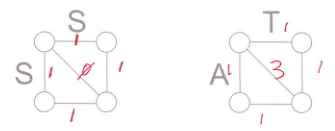
\includegraphics[width=\textwidth]{q2-weights}
	\end{center}
\end{figure}

\subsection{Shortest path}

Copying the weights from Figure \ref{fig:weights} we get Figure \ref{fig:Shortest:path}. The shorted path has length $1+0+0+1+0+1+1=4$. 
\begin{figure}[H]
	\begin{center}
		\caption{Shortest path}\label{fig:Shortest:path}
		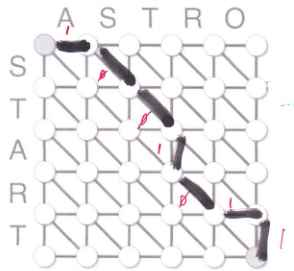
\includegraphics[width=0.6\textwidth]{q2-path}
	\end{center}
\end{figure}

% glossary
%\printglossaries

% bibliography go here

%\bibliographystyle{unsrt}
%\addcontentsline{toc}{section}{Bibliography}
%\bibliography{origins,wikipedia}

\begin{appendices}
	\section{Reference Implementation for Algorithm \ref{alg:find:maximum:independent:set}}\label{sect:ref:implementation}
	One way to implement Algorithm \ref{alg:find:maximum:independent:set} is with the following code.
	\lstinputlisting[language=Python]{mis.py}
\end{appendices}


\end{document}
